\section{Proofs of the exact moment results}
\label{app:proofs}

\subsection*{Proposition~\ref{prop:mean}}
\begin{proof}
  Condition on $r_j$. The other $G-1$ rewards are i.i.d.\ Bernoulli$(p)$ and, given $r_j$, are
  independent of $\score(y_j)$, so
  $\E[w(k, r_j)\score(y_j)] = \sum_{r} \Pr[r]\, W_r\, u_r$. Summing over $j$ and applying
  \eqref{eq:score-identity} gives $\E[z] = p\,(W_1 - W_0)\,u_1 = \lambda h$.
\end{proof}

\subsection*{Proposition~\ref{prop:cov}}
\begin{proof}
  Split $\E[z z^{\!\top}]$ into diagonal and off-diagonal terms. The diagonal contributes
  $G^{-1}[p Q_1 M_1 + (1-p) Q_0 M_0]$ with $M_r = S_r + u_r u_r^{\!\top}$. For $j \neq l$,
  condition on $(r_j, r_l)$ and on the count $m'$ among the remaining $G-2$ responses; the two
  scores are then conditionally independent, giving
  $\frac{G-1}{G}\sum_{a,b}\Pr[a]\Pr[b]\,C_{ab}\,u_a u_b^{\!\top}$, which collapses to
  $\frac{G-1}{G} p^2 (C_{11} - 2C_{10} + C_{00}) U$ by \eqref{eq:score-identity}. Subtracting
  $\E[z]\E[z]^{\!\top} = \lambda^2 p^2 U$ completes the proof.
\end{proof}

\section{Reproducing the results}
\label{app:repro}

Every figure and table is regenerated from stored run records by
\texttt{analysis/figures.py} and \texttt{analysis/tables.py}, and so is every headline number in
the prose: they are emitted as macros into \texttt{tables/numbers.tex} and referenced rather than
typed, so a rerun that moves a number moves it in the text as well. Each run writes a manifest holding the configuration, its hash, the commit the
code was at, and the interpreter and platform it ran on.

The exactness tests in \texttt{tests/} check every analytic result in Section~\ref{sec:theory}
against brute-force enumeration, and check the batched estimator against the reference
implementation term by term. Theorem~\ref{thm:adjoint} is additionally checked against the same
quantity assembled the expensive way, by building $S_T$ explicitly and forming
$\nabla M^{\!\top} S_T \nabla M$, and Proposition~\ref{prop:potential} against the measured
asymmetry of $\mathcal{J}$, which is $3\times10^{-10}$ across the estimator family, at the finite-difference
floor.

\paragraph{Evaluation randomness, and a bracket instead of a rerun.} Recovering a seed term from
the spread of an estimated score means subtracting the evaluation's own binomial variance, and that
subtraction assumes each run drew its own evaluation. The seven-billion runs were scored before we
noticed this, sharing one draw. Re-scoring them costs hours at that size, and is unnecessary: shared
evaluation noise is common to every run and so drops out of the variance between them, while
independent noise adds to it, which brackets the seed term between the observed spread and the
binomially corrected one whatever was actually shared. At $7$B those two ends differ by $0.3\%$,
because the binomial term is small against a spread that large. The smaller model was re-run with
independent draws, where the correction matters more.

\paragraph{One thing that was not reproducible, and now is.} The LoRA adapters are attached by
\texttt{mlx\_lm}, which draws their $A$ matrices from a generator that is not seeded by default.
Every process therefore began from a different parameterisation. The policy was the same either way,
because the $B$ matrices start at zero, and every seed within a run shares one initialisation, so
the spreads reported here are unaffected: the runs being compared differ only in rollout randomness,
as claimed. What was affected is repetition. Rerunning the same configuration gave different
numbers, which we noticed when a rerun of one experiment disagreed with itself. The initialisation
is now seeded from the run's configuration, and the released tests check that two attachments at one
seed agree and that two seeds do not.

\paragraph{What each thing costs.} Everything here ran on one Apple M4 laptop with $24$\,GB of
unified memory, and the costs are worth stating because they bound what a reader can repeat. The
enumerable-policy experiments are CPU work and finish in minutes; the $\numForecastSettings$-setting
forecast grid, which trains $\numForecastSeeds$ runs in each of them, takes about half an hour. The
populations of small transformers take a few hours each. On the pretrained models the arithmetic
changes: a single Qwen2.5-0.5B run of twelve updates takes about three minutes and its backward
pass about ten, while one Qwen2.5-7B run of twenty updates takes around an hour, so the eight-seed
measurement at $7$B is most of a day. That last figure is the reason this paper stops where it
does.

\paragraph{Using the backward pass elsewhere.} Algorithm~\ref{alg:forecast} needs two things from
a training run and nothing else: the variance across prompts of the batch gradient projected onto a
direction, and a Jacobian-vector product of the mean update field with that direction. The released
code states that as a protocol rather than a class hierarchy, so a trainer in another framework
implements two methods and reuses the recursion. Two implementations ship with it, one for
enumerable policies where every term is exact and one for a pretrained model through MLX. Both are
tested against systems whose answer is available in closed form: the protocol against linear
Gaussian recursions, and the pretrained-model implementation against a stand-in with the same
interface whose mean update field is a fixed linear map, which exercises the finite-difference
Hessian-vector product without needing a model to run it on.

One numerical detail is worth recording. The difference step $\epsilon$ has a floor set by the
precision the weights are held in: below roughly $10^{-4}$ in float32 the two evaluations cancel
into rounding error rather than into a derivative. We use $10^{-3}$, which sits above that floor and
well below the scale on which the gradient field bends.

\paragraph{A claim index.} The released code carries \texttt{docs/claims.md}, which lists every
claim in this paper against the experiment that produced it and how strongly it is supported:
exact, measured with an interval, observed without one, or a negative result. It also lists what we
withdrew and what we do not claim. It is written for a reader who distrusts one particular number
and wants to find its source without reading the code.

\paragraph{Which experiment produces what.}
\begin{itemize}\itemsep1pt
  \item \texttt{p1\_propagation}: the covariance recursion against Monte Carlo
    (Table~\ref{tab:propagation}, Figure~\ref{fig:teaser} right).
  \item \texttt{p2\_metric\_forecast}: the prospective forecast
    (Table~\ref{tab:forecast}, Figures~\ref{fig:teaser} left and \ref{fig:forecast}).
  \item \texttt{p3\_memory\_sources}: attribution and the memory horizon
    (Figure~\ref{fig:sources}, Section~\ref{sec:exp-forecast}).
  \item \texttt{p4\_linearity}: the linearisation residual (Section~\ref{sec:exp-linearity}).
  \item \texttt{p5\_adam\_lift}: the lifted recursion (Table~\ref{tab:adam-lift}).
  \item \texttt{p6\_spectrum}: the spectrum of the transfer operator (Table~\ref{tab:spectrum}).
  \item \texttt{s1}, \texttt{s3}, \texttt{s5}: seed divergence on transformers and on a pretrained
    model (Figures~\ref{fig:reconvergence} and \ref{fig:real-seeds}).
  \item \texttt{s6\_scale}: the seven-billion-parameter measurements
    (Section~\ref{sec:exp-scale}).
  \item \texttt{s7\_real\_forecast}: the backward pass on a pretrained model, and
    \texttt{power.py} the simulation of what that design can resolve
    (Appendix~\ref{app:power}).
  \item \texttt{s8\_null}: the same run with the reward replaced by a coin
    (Table~\ref{tab:signal}, Figure~\ref{fig:null}).
  \item \texttt{a}, \texttt{b}, \texttt{c}, \texttt{d}, \texttt{t}: the estimator, allocation and
    cost-model results of Section~\ref{sec:applications}.
\end{itemize}

The exact-tier experiments run in minutes on a laptop CPU. The pretrained-model experiments need
Apple Silicon and MLX; the seven-billion-parameter runs need about $24$\,GB of unified memory, and
the eight-seed sweep takes several hours.

\section{What the real-model design can resolve}
\label{app:power}

The seed spread of a score estimated from a finite evaluation is recovered by subtracting the
evaluation's own binomial variance from the observed spread across runs. That is a difference of
two noisy quantities, and below some true spread it is not distinguishable from zero. Reporting a
number from it without knowing where that boundary lies would be reporting noise.

\begin{table}[t]
  \centering
  \footnotesize
\setlength{\tabcolsep}{4pt}
\begin{tabular}{@{}lcccc@{}}
\toprule
& \multicolumn{2}{c}{6 runs} & \multicolumn{2}{c}{8 runs} \\
\cmidrule(lr){2-3} \cmidrule(lr){4-5}
true s.d. & resolved & estimate & resolved & estimate \\
\midrule
0.000 & 50\% & 0.000 & 46\% & 0.000 \\
0.010 & 58\% & 0.007 & 72\% & 0.009 \\
0.020 & 83\% & 0.018 & 88\% & 0.018 \\
0.040 & 99\% & 0.034 & 99\% & 0.039 \\
0.080 & 100\% & 0.069 & 100\% & 0.076 \\
\bottomrule
\end{tabular}
  \caption{Simulating the design as run, with $48$ held-out questions and $16$ samples each at a
  pass rate near $0.35$, over a range of true seed spreads. \emph{Resolved} is the fraction of trials in
  which the subtraction returns something positive; \emph{estimate} is the median of what it
  returns.}
  \label{tab:power}
\end{table}

Three readings from Table~\ref{tab:power}, and the first is a warning about the method rather than
about the data. At a true
spread of zero the subtraction still returns a positive number in about half of trials, because a
difference of two noisy variances is positive half the time. A non-zero reading is therefore not by
itself evidence of a seed spread; the interval is.

Second, the design resolves what it needs to. At a true spread of $0.02$ the subtraction recovers
something in $88\%$ of trials at eight runs and lands at a median of $0.018$; at $0.04$ it succeeds
essentially always. Those bracket the forecast we make.

Third, the bootstrap interval is anti-conservative here: its coverage of the true value runs from
$68\%$ to $88\%$ rather than the nominal $95\%$, which is the percentile bootstrap applied to a
variance difference at small $n$. We report the intervals because they are far more informative
than a point estimate, and note that they are narrower than they should be.

\section{The estimator family as a table}
\label{app:family}

Because the advantage depends only on $(k, r)$, an estimator is a $(G+1) \times 2$ array, and the
moments in \eqref{eq:contractions} are contractions of that array against a binomial distribution.
This is what makes the exact treatment cheap: no sampling is involved in evaluating
$\lambda(p, G)$, $Q_r$ or $C_{ab}$ for any member of the family, at any group size.


\section{Noise terms across task families}
\label{app:cross-family}

The corollary relating within-prompt noise to the reward histogram assumes a shared score
scale, which holds within a task family and not between families of different answer shape.
Table~\ref{tab:real} and Figure~\ref{fig:real-model} make the size of that effect explicit.

\begin{table*}[t]
  \centering
  \small
  \begin{tabular}{lcccccc}
\toprule
corpus & pass rate & $\E[p(1-p)]$ & $\tau_b$ & $\tau_w$ & $G^{*}$ & $\tau_w/\E[p(1-p)]$ \\
\midrule
count letter & 0.280 & 0.178 & 4.35e+02 & 1.16e+04 & 6.15 & 0.27 \\
nth word & 0.326 & 0.138 & 4.88e+03 & 2.01e+04 & 3.03 & 0.61 \\
add two & 0.546 & 0.062 & 1.29e+04 & 3.55e+04 & 2.66 & 2.40 \\
mixed & 0.193 & 0.071 & 4.31e+03 & 1.20e+04 & 2.67 & 0.71 \\
\bottomrule
\end{tabular}
  \caption{Noise terms measured on a pretrained model. The last column would be constant if the
  score scale were shared across families; it is not, and it is not meant to be.}
  \label{tab:real}
\end{table*}

\begin{figure}[t]
  \centering
  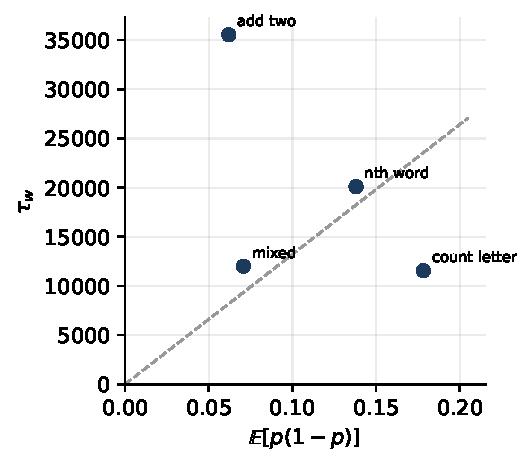
\includegraphics[width=0.95\linewidth]{figures/real_model.pdf}
  \caption{Within-prompt noise against the reward histogram across corpora, with a single fitted
  scale. The scatter is the score scale differing between task families.}
  \label{fig:real-model}
\end{figure}
